\documentclass[dvipdfmx,autodetect-engine,titlepage]{jsarticle}
\usepackage[dvipdfm]{graphicx}
\usepackage{ascmac}
\usepackage{fancybox}
\usepackage{listings}
\usepackage{plistings}
\usepackage{itembkbx}
\usepackage{amsmath}
\usepackage{svg}
\usepackage{url}
\usepackage{graphics}
\usepackage{listings,jvlisting}

\textheight=23cm
\renewcommand{\figurename}{図}
\renewcommand{\tablename}{表}
\newenvironment{code}
{\vspace{0.5zw}\VerbatimEnvironment  
\begin{screen} 
\baselineskip=1.0\normalbaselineskip
 \begin{Verbatim}}
{\end{Verbatim}
\baselineskip=\normalbaselineskip
 \end{screen}\vspace{0.5zw}} 

\title{情報理工学部 SNコース 2回\\
材料と化学\\
}
\author{2600200443-6\\Yamashita Kyohei\\山下 恭平}
\date{Jan 30 2022}

\begin{document}

\maketitle

\section{概要}
プラスチックの社会問題について取り上げ調査し、プラスチックの今後について考察
する。

\section{プラスチックの歴史}
19世紀以前、世の中にプラスチックが存在しなかった頃、人々は象牙や宝石などの
天然素材を必要な形に形成し利用してきた。しかし、天然素材は供給が常に不安定で
合ったとされている。19世紀に入ってからは化学が発展したこともあり半合成のプラスチック
が生活へと普及していく。天然ゴムに硫黄を加えた硬質ゴムや、天然の木綿に硝酸
などを反応させたセルロイドがその例である。しかし、この頃にはすでに、ポリ塩化
ビニルやポリスチレンは開発されていた。そして、20世紀に突入してからは合成
プラスチックの時代である。世界で初めて商標登録されたプラスチックは科学者
ベークランドによって開発されたフェノール樹脂「ベークライト」である。ベークラ
イトは電気絶縁性、耐熱性をもち人々の生活に大きく浸透していった。1926年に
化学者へルマン・スタウディンガーがポリマーが長い鎖状分子から出来ているというこ
とを発見し、プラスチックは大きく成長していく。1930年にはポリエチレンが1934年
にはアクリル樹脂が工業化し1938年にはナイロンが誕生した。第二次世界大戦では
様々なプラスチックが利用された。現代では、非常に多くのプラスチックが誕生し
私達の生活において必要不可欠なものとなっている。中には、形状を記憶するものや
、電気を通すもの、生体に適合するものなど、プラスチックの用途がかなり多岐に
渡っていることがわかる。*(1)(2)

\section{プラスチックが引き起こす問題}
プラスチックが日常生活において必要不可欠となる一方で、プラスチックは
重大な環境問題を引き起こしている。その一つが「海洋プラスチック問題」である。
この問題に大きくフォーカスが当てられるようになったのは2016年の世界経済フォー
ラムで以下のことが発表されたからである。

\begin{quote}
  \begin{math}
    ・世界のプラスチック生産量は1964年~2014年の50年間で20倍以上に急増。今後、20年間でさらに倍増
    する見込み。\\
    ・毎年少なくとも800万トン分のプラスチックが海に流出。\\
    ・海のプラスチック量は、2050年までには魚の量を上回る計算 \quad\quad-(3)
  \end{math}
\end{quote}
世界中でプラスチックが生産、使用されるようになったことで、その多くのゴミが海に
捨てられているのである。捨てられたプラスチックゴミの中には、ビニール袋、
釣り糸、漁猟用網などの丈夫で大きいものもあり、鳥や亀、魚などの海洋生物が、
誤飲してしまったり、網に絡まり溺死するといった事態が多く起きている。さらに
大きな問題は、捨てられたプラスチックは波や紫外線により大きさ5mm以下の「
マイクロプラスチック」になることである。当然海洋の生物達はこのマイクロプラスチック
を飲んでしまう。このことによって生物にどのような影響が出るのかを示した
研究が磯辺によって以下の様に示されている。

\begin{quote}
  \begin{math}
    図1は既往研究60編の結果である(Isobe etal., 2019)。縦軸は飼育水槽に混ぜたプラスチッ
    クビーズの濃度で、横軸には混ぜたビーズのサイズ(直径)を示す。プロットの位置は、水槽
    内の飼育生物に障害(成長障害や摂食障害、死亡率の上昇など)が発現した濃度とサイズの組
    み合わせである。これまで、濃度が1000 mg/m^3程度で障害を確認した実験が多い。すなわち、
    この程度にMPが浮遊する海域であれば、そこに棲む生物には、誤食したMPにより何らかの
    障害が現れることを示唆する^{(4)(5)}
  \end{math}
\end{quote}

\begin{figure}[h]
  \centering
  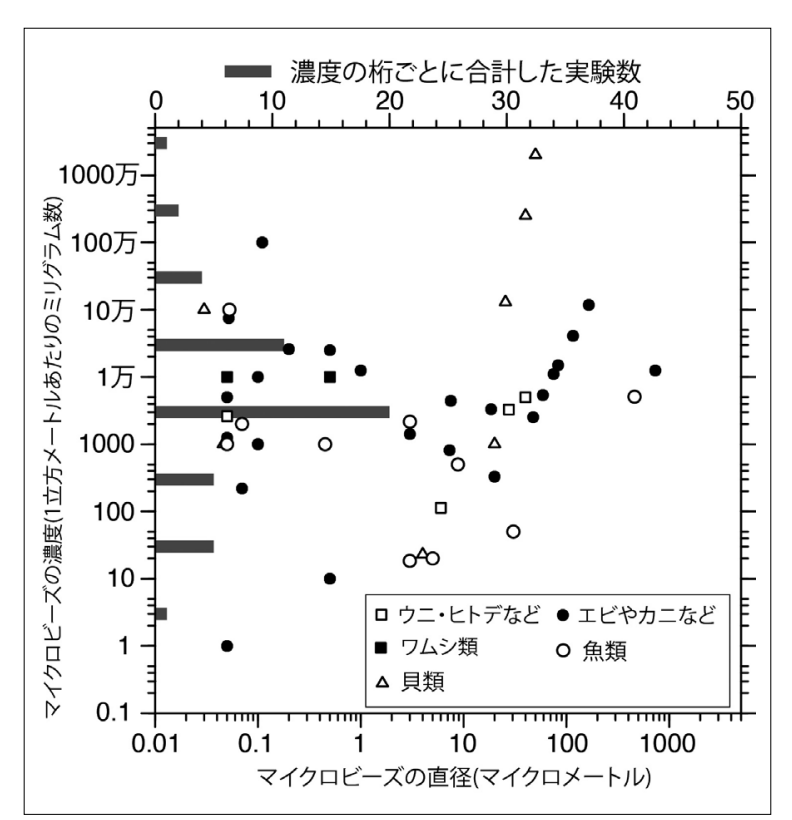
\includegraphics[scale=0.4]{SS1.png}
  \caption{マイクロプラスチックの粒子毒性実験結果}
\end{figure}

このように私たちが捨てるプラスチックによって多くの海洋生物に影響が出ていることが
わかった。また、日本の海岸には大量のプラスチックごみが打ち上げられており、
この問題に対しての意識が世界中の人々にとってまだ薄いことも大きな問題である。

\section{プラスチックのこれから}
この環境問題に対して、今後どのように取り組みが行われていくのかを考えていく。
先ほども述べた通り、プラスチックは私達の生活に必要不可欠のものであるので、
プラスチックを使用禁止にするという対策は取られることがないだろう。しかし、
プラスチックの使用量を減らすという努力は多くの企業ですでに行われていることで
ある。流通新聞の記事では。

\begin{quote}
  \begin{math}
    プラスチックの使用削減を企業に促す「プラスチック資源循環促進法」の20
    22年4月施行を控え、小売りや外食チェーンが対応を急いでいる。ファミリーマ
    ートは柄に穴を空けたスプーンを導入し、スターバックスコーヒージャパンはストローすべて
    を紙製に切り替えた。有料化への動きは鈍いようで、紙や木製への転換などで「減プラ」を
    目指す企業が目立つ。^{(6)}
  \end{math}
\end{quote}

スターバックス、ファミリーマート、KFC、イオン、ミニストップ、ハーゲンダッツ
といった大きな企業が次々に「減プラ」を行っており、私達の生活にも少し変化が
現れ出している。また、ユニクロ、無印良品といった企業では、積極的にプラスチック
の再利用が行われている。最近ではSDGsの14番で「海の豊かさを守ろう」として、
よく耳にすることも増えてきた。少しずつであるが確実に「減プラ」「リサイクル」
といった動きが私達の生活に溶け込んできており、今後数十年の間は成長し続けると
私は考えている。しかし、プラスチックの生産量を減らすだけでは問題解決はしないのは
明らかである。なので今後は、プラスチックを再利用する多くの技術が生まれると同時に、
プラスチックを「分解」する新しい技術の開発が進んでいくと私は考えている。
プラスチックを分解することが可能になれば、海でマイクロプラスチックとして
残り続ける問題は解決し、石油から生成したプラスチックを再び自然に返すことが
できるので、エネルギー問題についても大きな役割を果たすと考えられる。しかし、
プラスチックを「分解」するということはかなり難しいことであるので。私達
一人一人が日頃から、ゴミは分別することや、リサイクルBOXに衣類等を
持っていくなど、小さなことかもしれないが、意識を持って行動すること
が問題解決への第一歩であると私は考えている。

\section{参考文献リスト}

(1) 岳川 有紀子, 「プラスチックってなんだろう?: 歴史を紐解きながら考える」
 , 『化学と教育』, 2010\\
 \qquad\quad 4号58巻, p176 - p177\\

(2) 株式会社KDA, プラスチック専門サイト, \url{https://www.kda1969.com/study/study_pla_history.htm}\\

(3) 世界経済フォーラム(ダボス会議), 2016年1月, 海洋ごみに関する報告書\\

(4) Isobe, A. et al., Nature Communications, 10: 417, 2019\\

(5) 磯辺 篤彦. 「海洋の環境問題の観点から ─海洋プラスチック汚染」, 『学術の動向』, 2021, 1号26巻\\
\qquad\quad p48 - p50\\

(6)「スプーン類をエコに」義務付けへ、減プラ、有料化は慎重、外食など、木・紙製へ転換。\\
\qquad\quad 『日経MJ(流通新聞)』, 2021/11/19\\
\qquad\quad 日経テレコン21, \url{https://t21.nikkei.co.jp/g3/CMNDF11.do}\\

\end{document}

